\section{SchIM Implementation}
    As previously mentioned, SchIM is a PLIM module that performs a memory loop-back through the PL side similarly to \cite{PLIM20}.
    The objective of the module is to arbitrate the access of the bus to the main memory between the different cores of the PS side at the transaction level by enforcing a given policy.
    Roughly, the module receives transactions from the PS side, acknowledges them and finally repeat them with the main memory as destination.
    The exact order in which inter-core transactions are being repeated is decided by an embedded on-chip hardware scheduler.

    The present section exposes how SchIM interacts with the remaining of the systems in \ref{subsec:communication-scheme}, how its internal logic enforces transaction scheduling policies in \ref{subsec:micro-arch} and finally, an example of the transaction life cycle within the SchIM module is provided in \ref{subsec:transaction-life-cycle}.

    \subsection{Altered communication scheme}
        \label{subsec:communication-scheme}
        In order to achieve the objective of re-ordering transactions, one must alter the standard AXI communication scheme explained in the subsection \ref{subsec:axi_transaction_scheme}.
        To this end, we instantiate a in-between the master and the slave a pass-through module named SchIM as depicted in figure \ref{fig:SchIM_transaction_scheme_figure}.
        This module is the one in charge of the re-ordering of the transactions and does so by intercepting on the fly the transactions emitted by the masters before they reach the desired slaves.
        As shown in the figure \ref{fig:SchIM_transaction_scheme_figure}, only the phases instantiated by the masters (i.e. address phase on AW and AR and the data phase on W) are intercepted for re-ordering by SchIM.
        The introduction of SchIM has a direct consequence on the overall communication scheme. Indeed, while the response phases on channels R and B remain unchanged, the address and data phases are duplicated.
        Consequently, a write transaction will start exactly as in the standard AXI scheme with its address phase \circled{1} and data phase \circled{2}.
        These two transactions are buffered within the SchIm module in \circled{3} and only repeated when decided by the latter's internal logic.
        This release of the transaction leads to the initialisation of two new address and data phase \circled{4} and \circled{5}.
        Finally, the response phase \circled{6} goes directly from the slave to the master without being intercepted.
        The same modifications apply to the transmissions of read transactions as the address phase \circled{1'} is being buffered in \circled{2'} for some time before being re-emitted in \circled{3'}.
        As for the writing, the response phase \circled{4'} is not intercepted by SchIM.

        \begin{figure}
            \centering
            \begin{tikzpicture}[scale=0.5, every node/.style={scale=0.5}]
    % Module Master
    \draw ( 0.0, 0.0) -- ++( 2.0, 0.0) -- ++( 0.0, 5.25) -- ++( -2.0, 0.0);
    \node[rotate=90] at (0.25, 2.5) {\large MASTER};
    % Module Slave
    \draw (13.0, 0.0) -- ++(-2.0, 0.0) -- ++( 0.0, 5.25) -- ++( 2.0, 0.0);
    \node[rotate=270] at (12.75, 2.5) {\large SLAVE};
    % Module SchIM
    \draw ( 5.5, 2.25) rectangle ++( 2.0, 3.00) node [pos=.5] {\large SchIM};
    \draw[red] ( 6.25, 3.0) circle [radius=0.2] node {3};
    \draw[red] ( 6.75, 3.0) circle [radius=0.2] node {2'};
    % AW channel Master to SchIM
    \node at ( 1.5, 4.50) {AW};
    \draw ( 2.0, 4.25) rectangle ++( 3.5, 0.5);
    \draw ( 4.0, 4.25) rectangle ++( 0.5, 0.5)  node[pos=.5] {A};
    \draw[-{Stealth}] ( 4.5, 4.5) -- ++( 0.5, 0.0);
    \draw[red] ( 5.25, 4.5) circle [radius=0.2] node {1};
    \node at ( 11.5, 4.50) {AW};
    % W channel Master to SchIM
    \node at ( 1.5, 3.75) {W};
    \draw ( 2.0, 3.50) rectangle ++( 3.5, 0.5);
    \draw ( 2.5, 3.50) rectangle ++( 0.5, 0.5)  node[pos=.5] {D};
    \draw ( 3.0, 3.50) rectangle ++( 0.5, 0.5)  node[pos=.5] {...};
    \draw ( 3.5, 3.50) rectangle ++( 0.5, 0.5)  node[pos=.5] {D};
    \draw[-{Stealth}] ( 4.0, 3.75) -- ++( 0.5, 0.0);
    \draw[red] ( 4.75, 3.75) circle [radius=0.2] node {2};
    \node at ( 11.5, 3.75) {W};
    % AR channel Master to SchIM
    \node at ( 1.5, 3.00) {AR};
    \draw ( 2.0, 2.75) rectangle ++( 3.5, 0.5);
    \draw ( 4.0, 2.75) rectangle ++( 0.5, 0.5)  node[pos=.5] {A};
    \draw[-{Stealth}] ( 4.5, 3.0) -- ++( 0.5, 0.0);
    \draw[red] ( 5.25, 3.0) circle [radius=0.2] node {1'};
    \node at ( 11.5, 3.0) {AR};
    % AW channel SchIM to Slave
    \draw ( 7.5, 4.25) rectangle ++( 3.5, 0.5);
    \draw ( 9.5, 4.25) rectangle ++( 0.5, 0.5)  node[pos=.5] {A};
    \draw[-{Stealth}] ( 10.0, 4.5) -- ++( 0.5, 0.0);
    \draw[red] (10.75, 4.5) circle [radius=0.2] node {4};
    % W channel SchIM to Slave
    \draw ( 7.5, 3.50) rectangle ++( 3.5, 0.5);
    \draw ( 8.0, 3.50) rectangle ++( 0.5, 0.5)  node[pos=.5] {D};
    \draw ( 8.5, 3.50) rectangle ++( 0.5, 0.5)  node[pos=.5] {...};
    \draw ( 9.0, 3.50) rectangle ++( 0.5, 0.5)  node[pos=.5] {D};
    \draw[-{Stealth}] ( 9.5, 3.75) -- ++( 0.5, 0.0);
    \draw[red] (10.25, 3.75) circle [radius=0.2] node {5};
    % AR channel SchIM to Slave
    \draw ( 7.5, 2.75) rectangle ++( 3.5, 0.5);
    \draw ( 9.5, 2.75) rectangle ++( 0.5, 0.5)  node[pos=.5] {A};
    \draw[-{Stealth}] ( 10.0, 3.0) -- ++( 0.5, 0.0);
    \draw[red] (10.75, 3.0) circle [radius=0.2] node {3'};
    % B channel
    \node at ( 1.5, 1.5) {B};
    \draw ( 2.0, 1.25) rectangle ++( 9.0, 0.5);
    \draw ( 9.5, 1.25) rectangle ++( 0.5, 0.5)  node[pos=.5] {B};
    \draw[-{Stealth}] ( 9.5, 1.5) -- ++(-0.5, 0.0);
    \draw[red] ( 8.75, 1.5) circle [radius=0.2] node {6};
    \node at ( 11.5, 1.50) {B};
    % R channel
    \node at ( 1.5, 0.75) {R};
    \draw ( 2.0, 0.50) rectangle ++( 9.0, 0.5);
    \draw ( 8.0, 0.50) rectangle ++( 0.5, 0.5)  node[pos=.5] {D};
    \draw ( 8.5, 0.50) rectangle ++( 0.5, 0.5)  node[pos=.5] {...};
    \draw ( 9.0, 0.50) rectangle ++( 0.5, 0.5)  node[pos=.5] {D};
    \draw ( 9.5, 0.50) rectangle ++( 0.5, 0.5)  node[pos=.5] {B};
    \draw[-{Stealth}] ( 8.0, 0.75) -- ++(-0.5, 0.0);
    \draw[red] ( 7.25, 0.75) circle [radius=0.2] node {4'};
    \node at ( 11.5, 0.75) {R};
\end{tikzpicture}

            \caption{Caption}
            \label{fig:SchIM_transaction_scheme_figure}
        \end{figure}

    \subsection{Micro-architecture}
        \label{subsec:micro-arch}
        The SchIM module is composed of many sub-modules that can themselves be grouped into three different domains. In fact, as illustrated in figure \ref{fig:MemorEDF_module_schema}, one can distinguish the \emph{scheduling domain}, the \emph{queuing domain} and the \emph{interfacing domain}.

        The scheduling domain encompasses all the sub-modules that enable arbitration of the bus between the transactions issued by the different cores of the PS side. Hence, this domain boasts several transaction schedulers implemented at the hardware level.
        The scheduling policies offered by SchIM include Fixed Priority (FP), Time Division Multiple Access (TDMA), Earliest Deadline First (EDF), Least Laxity First (LLF) and MemGuard (MG).
        Each of the parameters required by the aforementioned algorithms such as the priorities, the periods, the deadlines and the budgets are re-configurable at the run-time thanks to the inclusion of a configuration port.
        Finally, the scheduling domain is also the one in charge of the control of the remaining the SchIM module, driving and selecting the adequate signals and ensuring the coherence and integrity of the data.

        The queuing domain is in charge of the storing the incoming transactions emitted by the PS side.
        The motivation behind the use of queues is implied by the fact that all the masters located on the PS side share a common AXI bus (namely HPM0 as shown in figure \ref{fig:SchIM_overview_schema}).
        Therefore, in order to cancel the Round Robin arbitration policy applied in the PS side and in order to avoid that one high priority core is stalled by a lower priority one, each core is granted a queue within the SchIM module.
        Not only the queues act as containers and buffers for transactions, they also embed logic and provide information to the scheduling domain regarding their current state in order to avoid the queues to overflow or underflow similarly to the producer-consumer problem.
        As suggested by figure \ref{fig:MemorEDF_module_schema}, transactions are inserted to the adequate queues on the basis of the emitters identifier via the dispatcher module.
        Similarly, transactions are evicted from their queue, routed by the selector module and sent directly to the output of the module upon the action of the scheduling domain.

        The interfacing domain encompasses the sub-modules in charge of interfacing both the scheduling domain and the queuing domain with the remaining of the system using the AXI protocol.
        More accurately, three sub-modules compose this domain, the configuration port previously mentioned, the packetizer and the serializer.
        While the packetizer and the serializer serve the purpose of slave and master ports, they are also in charge of respectively transforming the AXI transactions into an equivalent packet and to transform these packets back to a AXI compliant transactions.
        The need for packetizing (i.e. flattening) the AXI transactions is driven by the necessity of storing transactions that are by nature serial within the queuing domain.
        For instance, a standard AXI transaction is composed of one address phase followed by a data phase which itself composed of multiple successive bursts.

        \begin{figure}
            \centering
            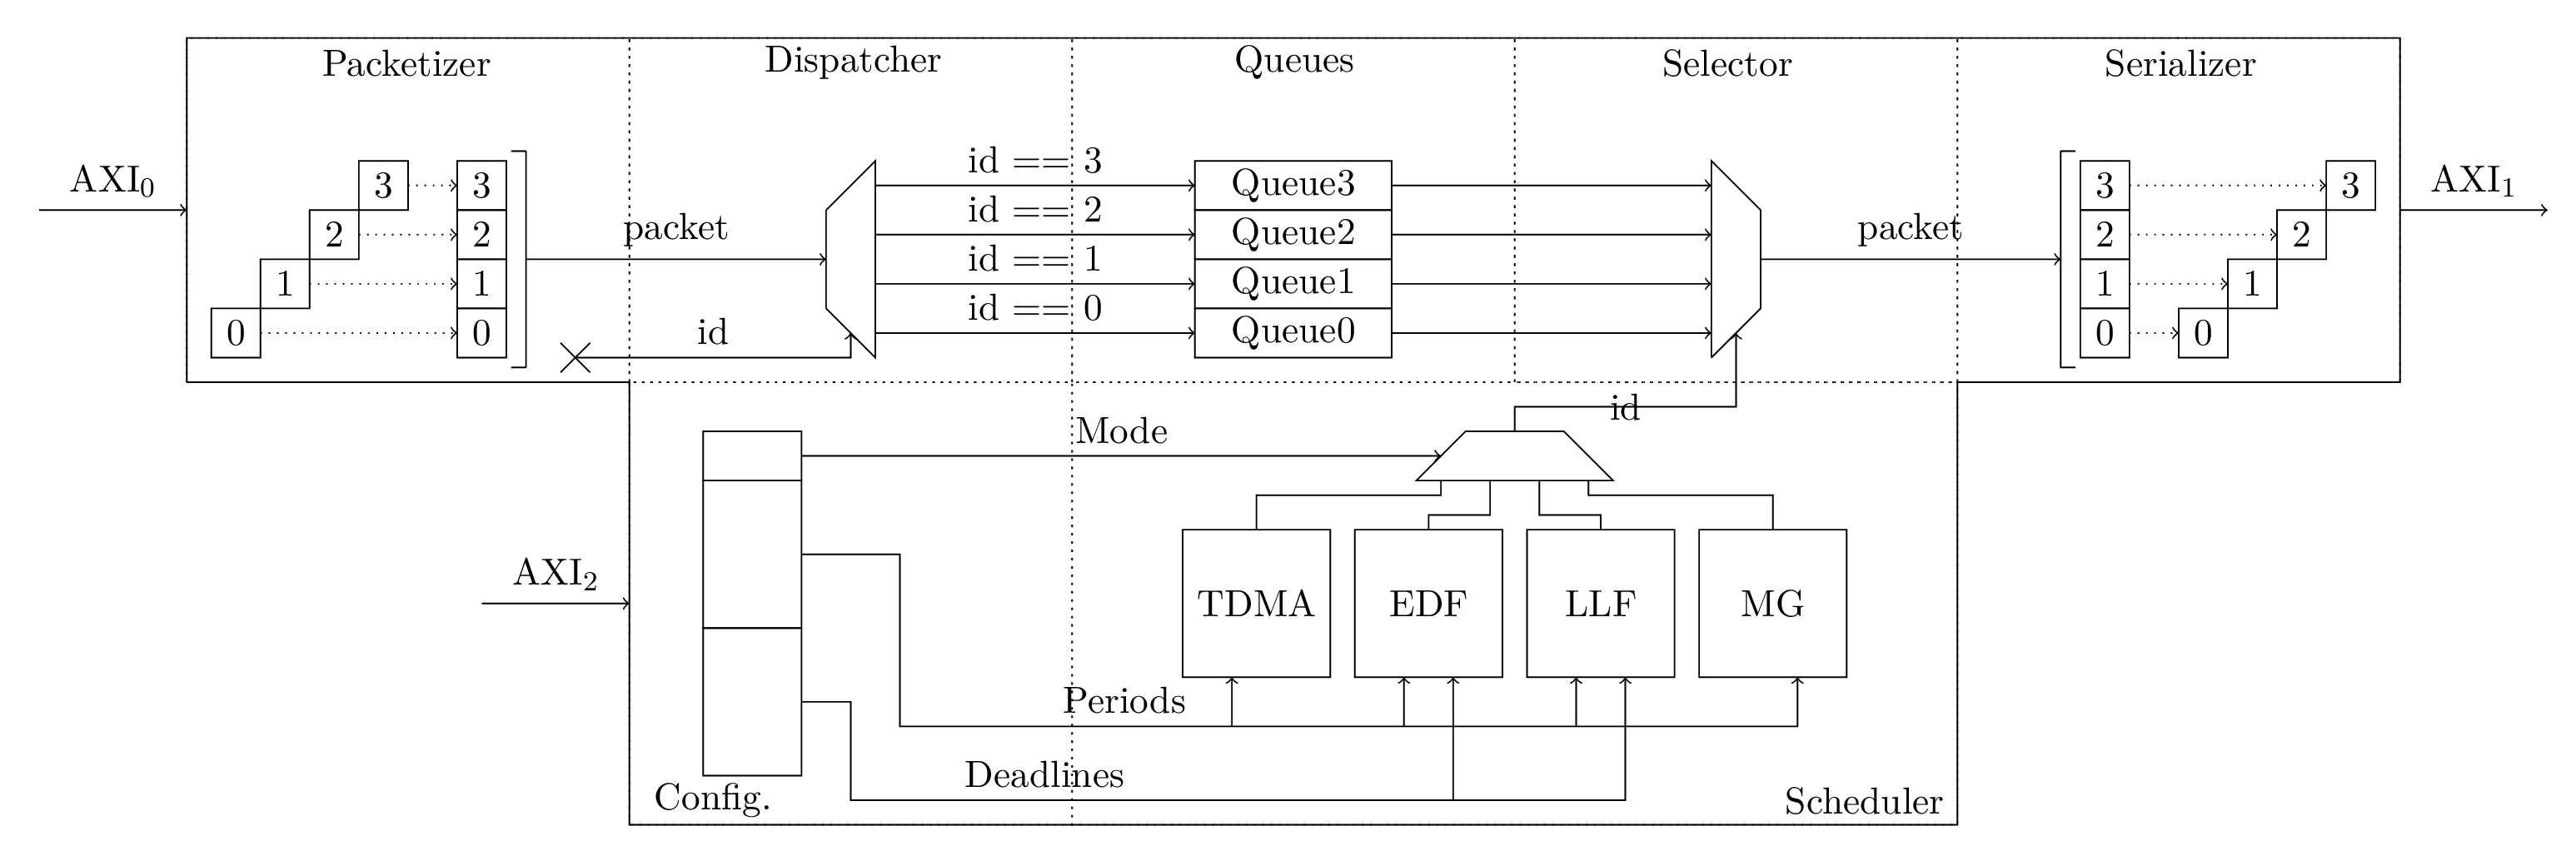
\includegraphics[scale=0.08]{images/MemorEDF_module_schema.png}
            \caption{Caption}
            \label{fig:MemorEDF_module_schema}
        \end{figure}
        
    \subsection{Embedded Schedulers}
        
        \subsubsection{Fixed Priority}
            The Fixed Priority scheduling module aims at enforcing prioritization of the traffic of the cores. The priority ordering is explicitly defined by the user through the configuration port. While SchIM only has four queues, 16 different levels of priority are offered. Note that, as it stands, the ordering is strict, meaning that two cores cannot be assigned with the same priority.
          
            The FP scheduling module only needs two information: the priority associated with each queue and whether a given queue contains at least one buffered transaction. Intuitively, the module logic consists in always considering the highest priority hence, a argmax function is implemented. However, lower priority queues must also be considered when higher priority queue do not have transactions. Consequently, the user defined priority is temporarily considered as 0 when its corresponding queue does not contain transaction.
        
        \subsubsection{Time Division Multiple Access}
            The Time Division Multiple Access (or TDMA) scheduling module provided by SchIM is a non-work conserving policy that splits the bus usage between the cores for given periods (also referred to as slots). The proposed embedded TDMA module enables the user to specify a different TDMA slot size for each core. The periods are expressed in clock cycles, enabling a fine grained granularity. The configuration port enables the end-user to specify and change the periods at runtime.
            
            The implementation of the modules relies on a single register used as a counter. In fact, we use this register to count the time elapsed in the current TDMA hyper-period (i.e., the sum of all the cores period) and is reset to 0 once this hyper-period reached. Alongside this register, a logic is there to determine in which core slot the counter actually is and to forward the information to the queue selector. The logic is able to determine the core to schedule by summing the period of each previous cores. Provided that the current value of the counting register is contain between the sum of the previous periods and the sum of the previous periods and the current one, the information forwarded to the remaining of the system will be the core id corresponding to the interval.
            \todo[inline]{DH: @DH TODO improve description!}
        
        \subsubsection{MemGuard}
            The proposed MemGuard transaction scheduling policy is inspired by the Software-based bus regulation technique ??. The latter has been proved to ensure memory isolation for all the cores involved. Unlike the original MemGuard, the proposed version does not rely on memory budgets and replenishment periods. Instead, it enforces inter-arrival time (i.e. a guaranteed minimal period) between two consecutive transactions emitted by a given core. This distinguishes our approach from \cite{Farshchi2020BRUBR}.
                    
            This scheduling module is implemented as follows. For each of the queues to schedule, the module has a register counting the time elapsed since the start of the period. Once this counter has reached the period set by the user (through the configuration port), the module checks if the queue corresponding to the core contains any transaction. In the case where a transaction is available in the corresponding queue, the latter is forwarded to the output of SchIM (i.e., the serializer) and the counting register is reset to 0. Otherwise, the counting register is blocked to the desired period until a transaction is available for scheduling in the corresponding queue, leading to the counting register to be reset to 0. Any tie between two cores is solved using a fixed priority arbitration defined by the user thanks to the configuration port. 

    \subsection{Transactions Life Cycle}
        \label{subsec:transaction-life-cycle}
        Let us consider a system with four cores (noted $C = \{c_{0}, c_{1}, c_{2}, c_{3}\}$) sending transactions $T = \{t_{0}, t_{1}, ..., t_{n}\}$ to the SchIM module.
        Consequently, the latter boasts four queues (noted $Q = \{q_{0}, q_{1}, q_{2}, q_{3}\}$) buffering the transactions under the form of packets $P = \{p_{0}, p_{1}, ..., p_{n}\}$ where $p_{i} = Packetizer(t_{i})~\forall i \in [0 : n]$.

        In the present example, we will assume $t_{1}$ as being the transaction under analysis.
        The latter is emitted by $c_{2}$ in direction of the SchIM module.
        The packetizer receives this transaction and, once the AXI protocol completed, transform it into an equivalent packet $p_{1} = Packetizer(t_{1})$.
        Following this transformation, the newly created packet is forwarded to the dispatcher which, thanks to the emitter's id embedded within the transaction, is re-routed to the corresponding queue $q_{2}$ (since emitted by $c_{2}$).
        After the insertion of $p_{1}$ in $q_{2}$, the state of the queuing domain is as follows: $q_{0}$ has two packets $p_{0}$ and $p_{k}$ and $q_{2}$ only has $p_{1}$.
        At this point, $q_{0}$ is considered for scheduling by the scheduling domain.
        In consequence, $p_{0}$ is forwarded to the serializer through the selector.
        Simultaneously to the reception of the packet by the serializer, the latter receives an activation signal from the scheduling domain informing the serializer that the packet is valid and that a transaction can be started.
        Similarly to the packetizer, the serializer will transform the packet $p_{0}$ back to its initial AXI transaction form $t_{0} = Serializer(p_{0})$.
        Thereafter, once the $t_{0}$ has been sent, the serializer will inform the scheduling domain via a signal, that he is ready to accept the next packet as input.
        Upon the reception of this signal, the scheduling domain will both re-direct the latter to the queue of the previous packet to indicate that it has been consumed and change the selected queue according to the scheduling policy so that the first packet of this queue can be forwarded to the serializer through the selector module.
        In the present example, the "consumed" signal forwarded by the scheduler is sent to $q_{0}$ which is then empty.
        At this instant, two scenarios are possible:
        \begin{enumerate}
            \item $q_{0}$ is still considered for scheduling following the selected scheduling policy. Therefore, as $q_{0}$ is empty, it outputs an "empty" signal received by the scheduling domain.
                  The latter then decides to not send any activation signal to the serializer because there is nothing left to transmit in the selected queue.
                  In other words, the access to the main memory is being stalled on purpose by the scheduling policy i.e. the scheduling policy is not work conserving.
                  For instance, such a scenario could happen in the case of TDMA or if all the queues are empty.
                  The logic will resume as soon as the selected queue is filled.
            \item $q_{2}$ is now considered instead of $q_{0}$ for scheduling.
                  In this case, the "consumed" signal is repeated to $q_{0}$ while the queue ID changes in order to select $q_{2}$.
                  This results in the packet contained inside $q_{1}$ to be forwarded to the selector.
        \end{enumerate}
